\documentclass[10pt]{beamer}
\usetheme{Boadilla}


\usepackage{amsmath}

\usepackage{graphicx}
\graphicspath{ {./images/} }

\title{ECEN 773 Project}
\subtitle{EKF With Parameter Estimation}
\author{Mark Petersen}
\institute{Brigham Young University}
\date{\today}


\begin{document}

\begin{frame}
\titlepage
\end{frame}


%%%%%%%%%%%%%%%%%%%%%%%%%%%%%%%%%%%%%%%%%%%%%%%%%%%%%%%%%%%%%%%%%%%%%%%%%%%%%%%%%%%%%%%%%%%%%%%%%%%%%%%%%%%%
%
%%%%%%%%%%%%%%%%%%%%%%%%%%%%%%%%%%%%%%%%%%%%%%%%%%%%%%%%%%%%%%%%%%%%%%%%%%%%%%%%%%%%%%%%%%%%%%%%%%%%%%%%%%%%

\begin{frame}
\frametitle{Outline}
\tableofcontents
\end{frame}

%%%%%%%%%%%%%%%%%%%%%%%%%%%%%%%%%%%%%%%%%%%%%%%%%%%%%%%%%%%%%%%%%%%%%%%%%%%%%%%%%%%%%%%%%%%%%%%%%%%%%%%%%%%%
%
%%%%%%%%%%%%%%%%%%%%%%%%%%%%%%%%%%%%%%%%%%%%%%%%%%%%%%%%%%%%%%%%%%%%%%%%%%%%%%%%%%%%%%%%%%%%%%%%%%%%%%%%%%%%

\section{Kalman Filter}
\subsection{Problem Statement}


 
\begin{frame}
  \frametitle{Problem Statement}

  Consider the LTI Discrete system

  \begin{align*}
  \mathbf{x}_{k+1} &= A\mathbf{x}_k + Bu_{k+1} + \mathbf{w}\\
  \mathbf{y}_{k+1} &= C\mathbf{x}_{k+1} + \mathbf{v}
  \end{align*}

  where $\mathbf{w}$ is process noise and $\mathbf{v}$ is observation noise with zero mean multivariate normal distribution with covariances $Q$ and $R$, $\mathcal{N}(0,Q)$, $\mathcal{N}(0,R)$. \\
  \hspace{10pt}

  and the observer

  \begin{align*}
  \mathbf{\dot{\hat{x}}}_{k+1} &= A\mathbf{\hat{x}}_{k} + Bu_{k+1}\\
  \mathbf{\hat{y}}_{k+1} &= C\mathbf{\hat{x}}_{k+1}
  \end{align*}

\end{frame}

%%%%%%%%%%%%%%%%%%%%%%%%%%%%%%%%%%%%%%%%%%%%%%%%%%%%%%%%%%%%%%%%%%%%%%%%%%%%%%%%%%%%%%%%%%

\subsection{Bayes' Inference}

\begin{frame}

  \frametitle{Bayes' Inference}

  $$p(x|y) = \frac{ p(y|x)p(x)}{p(y)} = \frac{\text{likelihood}\times \text{prior}}{\text{normalizing factor}} $$

\end{frame}


%%%%%%%%%%%%%%%%%%%%%%%%%%%%%%%%%%%%%%%%%%%%%%%%%%%%%%%%%%%%%%%%%%%%%%%%%%%%%%%%%%%%%%%%%%

\subsection{Prior}

\begin{frame}

  \frametitle{Prior}

  Let $\mathbf{x}_k$ be a multivariate normal random process at time step $k$ with mean $\hat{x}_k$ and covariance $P_k$,  $\mathcal{N}(\hat{x}_k,P_k)$ Then
 $$\mathbf{x}_{k+1|k} = A\mathbf{x}_k + Bu_{k+1} + \mathbf{w}$$ 
 $$\textbf{E}\{x_{k+1|k}\} = \hat{x}_{k+1|k} =  A\hat{x}_k + Bu_{k+1}$$
 $$\textbf{E}\{x_{k+1|k} -\hat{x}_k)(x_{k+1|k} -\hat{x}_k)^\top \} = P_{k+1|k} = AP_kA^\top + Q $$ 

 and the prior is

 $$p(x) = k_x\text{exp}\left( -\frac{1}{2}(\mathbf{x} - \hat{x})^\top P^{-1}(\mathbf{x} - \hat{x})\right) $$   
 where $k_x$ is a constant coefficient of a Gaussian PDF.

\end{frame}

%%%%%%%%%%%%%%%%%%%%%%%%%%%%%%%%%%%%%%%%%%%%%%%%%%%%%%%%%%%%%%%%%%%%%%%%%%%%%%%%%%%%%%%%%%


\subsection{Likelihood}

\begin{frame}

  \frametitle{Likelihood}

  Let $\mathbf{y}_k$ be a multivariate normal random process at time step $k$. Then
  $$\mathbf{y}_{k+1 | k+1} = C\mathbf{x}_{k+1} + \mathbf{v_k}$$

 and the likelihood is

 $$p(y|k) = k_y\text{exp}\left( -\frac{1}{2}(\mathbf{y} - Cx)^\top R^{-1}(\mathbf{y} - Cx)\right) $$   
 where $k_y$ is a constant coefficient of a Gaussian PDF.



\end{frame}


%%%%%%%%%%%%%%%%%%%%%%%%%%%%%%%%%%%%%%%%%%%%%%%%%%%%%%%%%%%%%%%%%%%%%%%%%%%%%%%%%%%%%%%%%%

\subsection{Posterior}

\begin{frame}

  \frametitle{Posterior}

  The posterior, $$p(x|y) = k_{xy}\text{exp}\left( -\frac{1}{2}(\mathbf{y} - Cx)^\top R^{-1}(\mathbf{y} - Cx)\right)\text{exp}\left( -\frac{1}{2}(\mathbf{x} - \hat{x})^\top P^{-1}(\mathbf{x} - \hat{x})\right) $$,

  is maximized when

  $$ \frac{\partial}{\partial x} \left[ -\frac{1}{2}(\mathbf{y} - Cx)^\top R^{-1}(\mathbf{y} - Cx) -\frac{1}{2}(\mathbf{x} - \hat{x})^\top P^{-1}(\mathbf{x} - \hat{x}\right] = 0$$

  i.e. when 

  $$ \hat{x} = \left( P^{-1} + C^\top R^{-1} C \right)^{-1}\left( P^{-1}\hat{x} + H^\top R^{-1}y\right) $$



\end{frame}


%%%%%%%%%%%%%%%%%%%%%%%%%%%%%%%%%%%%%%%%%%%%%%%%%%%%%%%%%%%%%%%%%%%%%%%%%%%%%%%%%%%%%%%%%%

\subsection{Kalman Filter}

\begin{frame}

  \frametitle{Kalman Filter}

  \begin{tabular}{cc}
  % \hline
  % 1 & 2
  \textbf{Predict} & \\
  Predicted (\textit{a priori}) state estimate & $\hat{x}_{k|k-1} = A\hat{x}_{k-1|k-1} + Bu_k$  \\
  Predicted (\textit{a priori}) error covariance & $P_{k|k-1} = AP_{k-1|k-1}A^\top + Q$ \\

  \textbf{Update} & \\
  Innovation & $z = y_k - C\hat{x}_{k|k-1}$ \\
  Innovation Covariance & $S_k = R + CP_{k|k-1}C^\top$ \\
  Kalman gain & $K_k = P_{k|k-1}CS_k^{-1}$ \\
  Updated (\textit{a posteriori}) state estimate & $\hat{x}_{k|k} = \hat{x}_{k|k-1} + K_k z$ \\
  Updated (\textit{a posteriori}) estimate covariance & $P_{k|k} = (I - K_kC)P_{k|k-1}$ 
  % \hline
  \end{tabular}  

  



\end{frame}

%%%%%%%%%%%%%%%%%%%%%%%%%%%%%%%%%%%%%%%%%%%%%%%%%%%%%%%%%%%%%%%%%%%%%%%%%%%%%%%%%%%%%%%%%%%%%%%%%%%%%%%%%%%%
%
%%%%%%%%%%%%%%%%%%%%%%%%%%%%%%%%%%%%%%%%%%%%%%%%%%%%%%%%%%%%%%%%%%%%%%%%%%%%%%%%%%%%%%%%%%%%%%%%%%%%%%%%%%%%

\section{Extended Kalman Filter}
\subsection{Problem Statement}
\begin{frame}

\frametitle{Problem Statement}

  \begin{align*}
  \mathbf{x} &= f(\mathbf{x},u) + \mathbf{w}\\
  \mathbf{y} &= C\mathbf{x} + \mathbf{v}
  \end{align*}

  where $\mathbf{w}$ is process noise and $\mathbf{v}$ is observation noise with zero mean multivariate normal distribution with covariances $Q$ and $R$, $\mathcal{N}(0,Q)$, $\mathcal{N}(0,R)$. \\
  \hspace{10pt}

\end{frame}

%%%%%%%%%%%%%%%%%%%%%%%%%%%%%%%%%%%%%%%%%%%%%%%%%%%%%%%%%%%%%%%%%%%%%%%%%%%%%%%%%%%%%%%%%%%%%%%%%%%%%%%%%%%%
\subsection{Extended Kalman Filter}
\begin{frame}

\frametitle{EXF Discrete}

  \begin{tabular}{cc}
  % \hline
  % 1 & 2
  \textbf{Predict} & \\
  Predicted (\textit{a priori}) state estimate & $\hat{x}_{k|k-1} = f(\hat{x}_{k-1|k-1},u_k)$  \\
  Predicted (\textit{a priori}) error covariance & $P_{k|k-1} = FP_{k-1|k-1}F^\top + Q$ \\

  \textbf{Update} & \\
  Innovation & $z = y_k - C\hat{x}_{k|k-1}$ \\
  Innovation Covariance & $S_k = R + CP_{k|k-1}C^\top$ \\
  Kalman gain & $K_k = P_{k|k-1}CS_k^{-1}$ \\
  Updated (\textit{a posteriori}) state estimate & $\hat{x}_{k|k} = \hat{x}_{k|k-1} + K_k z$ \\
  Updated (\textit{a posteriori}) estimate covariance & $P_{k|k} = (I - K_kC)P_{k|k-1}$ 
  % \hline
  \end{tabular} 

  where $F$ is the jacobian of $f(x,u)$ with respect to $x$. 

\end{frame}

\subsection{Parameter Estimation}

\begin{frame}

\frametitle{EKF Parameter Estimation}

Augment the states with the parameters s.t.

$$ x_{a} = 
\begin{bmatrix}
x \\
p
\end{bmatrix}
$$

and the system becomes 

  \begin{align*}
  \mathbf{x}_{a} &= f(\mathbf{x}_{a},u) + \mathbf{w}\\
  \mathbf{y} &= C\mathbf{x_{new}} + \mathbf{v}
  \end{align*}


\end{frame}

%%%%%%%%%%%%%%%%%%%%%%%%%%%%%%%%%%%%%%%%%%%%%%%%%%%%%%%%%%%%%%%%%%%%%%%%%%%%%%%%%%%%%%%%%%%%%%%%%%%%%%%%%%%%
%
%%%%%%%%%%%%%%%%%%%%%%%%%%%%%%%%%%%%%%%%%%%%%%%%%%%%%%%%%%%%%%%%%%%%%%%%%%%%%%%%%%%%%%%%%%%%%%%%%%%%%%%%%%%%
\section{Whirlybird}
\subsection{System}

\begin{frame}

\frametitle{System}

\begin{align*}
  x &= f(x,u) \\
  y &= C\mathbf{x}
\end{align*}

where 

\begin{align*}
 x &= [\phi, \theta, \psi, \dot{\phi}, \dot{\theta}, \dot{\psi}, Jx, Jy, Jz]^\top \\
 y & = [\phi, \theta, \psi]^\top \\
 f &: \mathbf{R}^9 \rightarrow \mathbf{R}^9 \\
 C &: \mathbf{R}^9 \rightarrow \mathbf{R}^3
\end{align*}


where $Jx, Jy, Jz$ are the moments of inertia and the parameters to be estimated.




\end{frame}

%%%%%%%%%%%%%%%%%%%%%%%%%%%%%%%%%%%%%%%%%%%%%%%%%%%%%%%%%%%%%%%%%%%%%%%%%%%%%%%%%%%%%%%%%%%%%%%%%%%%%%%%%%%%


\subsection{Observability Theorem}

\begin{frame}

\frametitle{Observability Theorem}

Using the non lienar system 

  \begin{align*}
  \dot{x} &= f(x)\\
  y &= Cx 
  \end{align*}

% \textbf{Inverse function theorem}: A differentiable multivariable function $y: \textbf{R}^n \rightarrow \textbf{R}^n$ is invertible in the neighborhood of a point $x_o$ as long as the jacobian of $y$ at $x_o$ is invertible. 

\textbf{Observability}: Let $\mathcal{O}_s$ be the observation space containing all repeated lie derivatives of $y$, then the system is locally observable in $x_o$ iff $\text{dim}(\frac{\partial{\mathcal{O}_s(x_o)}}{\partial x}) = n$. Where $n$ is the number of states. 

$$\mathcal{O}_s = 
\begin{bmatrix}
y = Cx\\
\dot{y}  = Cf(x)\\
\ddot{y} = C\frac{\partial f}{\partial x}f(x)\\
\vdots
\end{bmatrix}
$$

The rank of $\frac{\partial \mathcal{O}_s}{\partial x}$ for the WB is $9$. Thus observable at certain configurations. 


\end{frame}

%%%%%%%%%%%%%%%%%%%%%%%%%%%%%%%%%%%%%%%%%%%%%%%%%%%%%%%%%%%%%%%%%%%%%%%%%%%%%%%%%%%%%%%%%%%%%%%%%%%%%%%%%%%%


\section{Results}
\begin{frame}
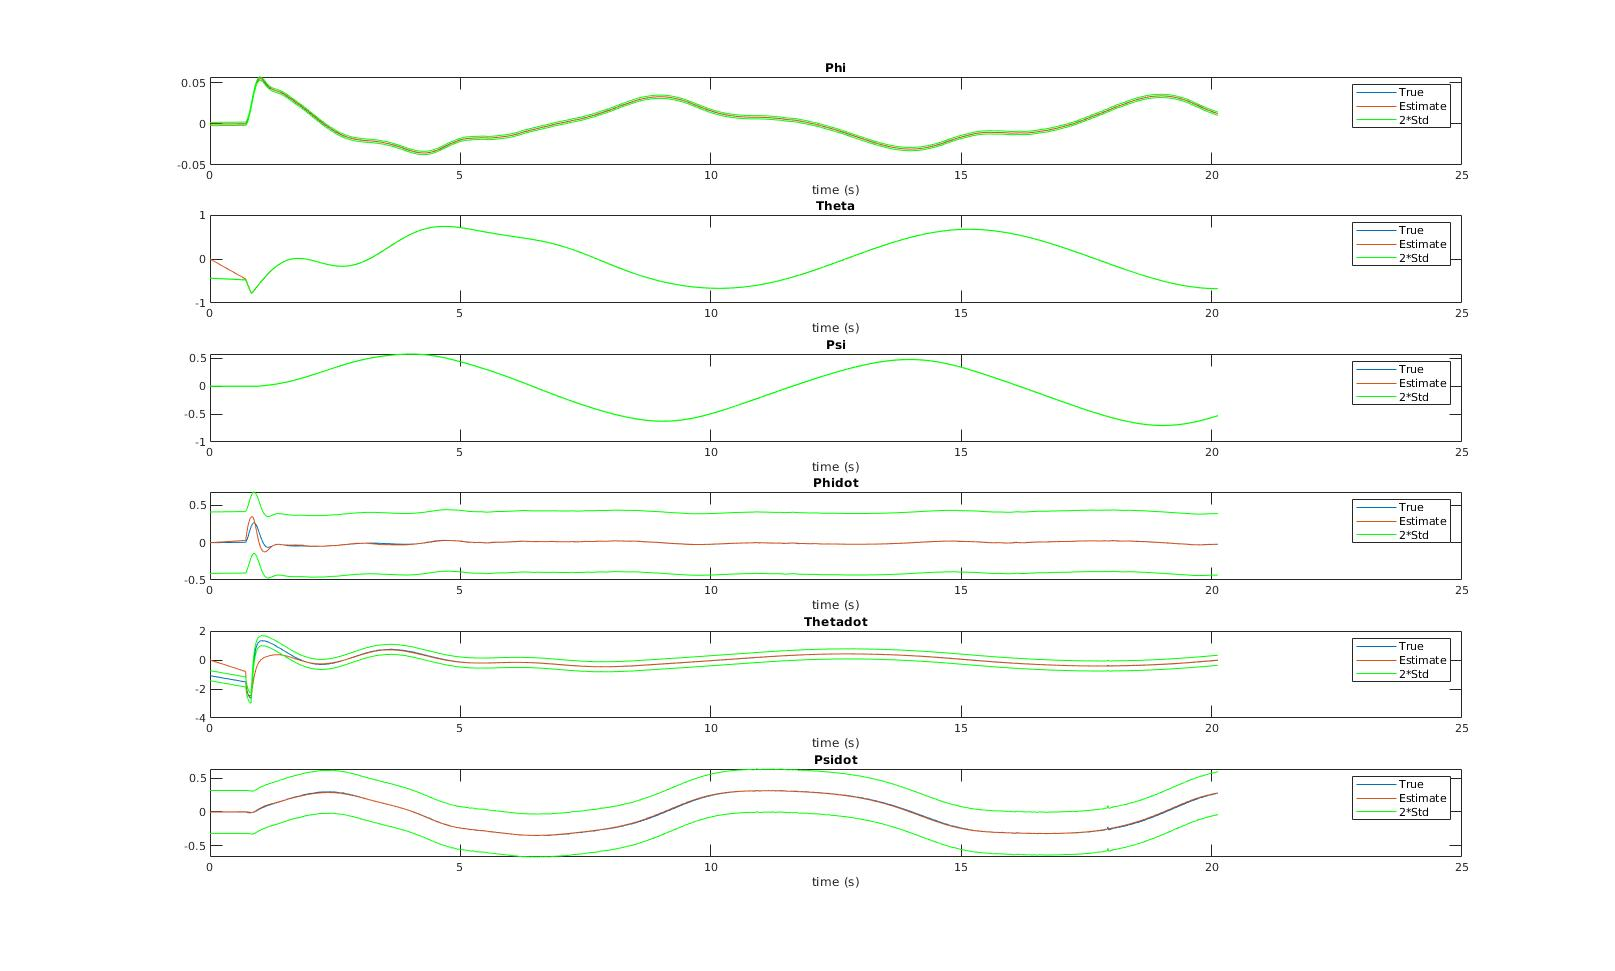
\includegraphics[width=0.8\textwidth,height=0.8\textheight]{images/states.jpg}
\end{frame}

\begin{frame}
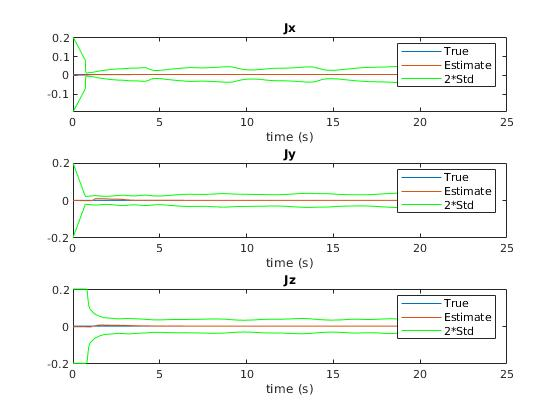
\includegraphics[width=0.8\textwidth,height=0.8\textheight]{Parameters}
\end{frame}

\begin{frame}
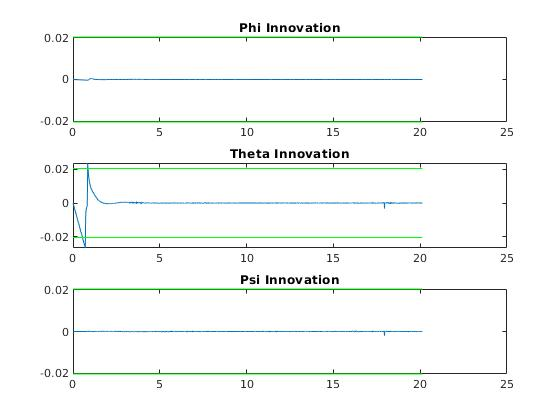
\includegraphics[width=0.8\textwidth,height=0.8\textheight]{innovation}
\end{frame}


\end{document}